\documentclass[tikz,border=2pt]{standalone}
\usepackage{amsmath}
\usepackage{pgfplots}
\pgfplotsset{compat=1.18}

\begin{document}
% Envelope theorem: the value function V(alpha) = max_x f(x; alpha) is the upper envelope of
% the curves alpha -> f(x; alpha) for fixed x; at alpha_0 it touches the curve of the optimal
% x*(alpha_0), so V'(alpha_0) = partial f / partial alpha at x*(alpha_0) — no need to track
% how x* itself moves.
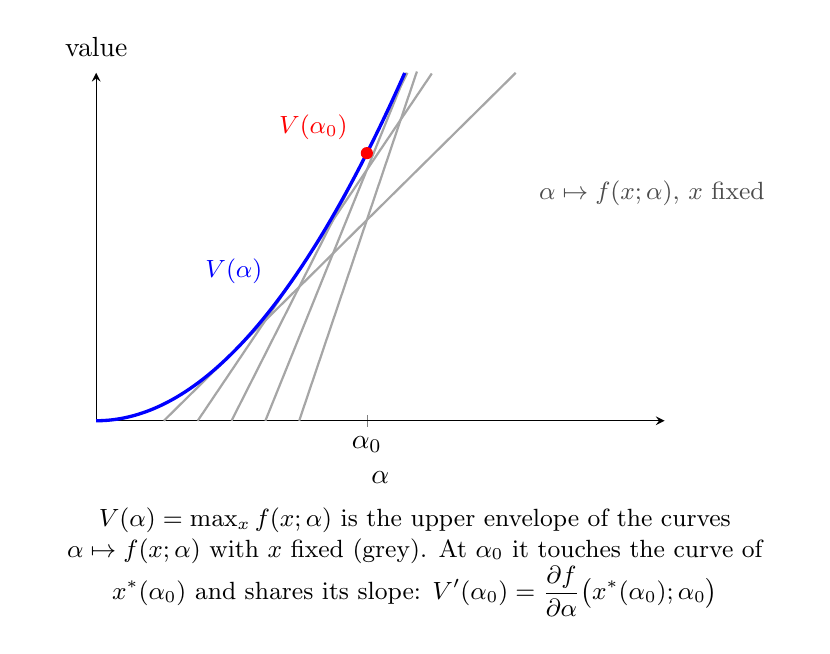
\begin{tikzpicture}
	\begin{axis}[
		axis lines=left, xmin=0, xmax=4.2, ymin=0, ymax=5.2,
		xtick={2}, xticklabels={$\alpha_0$}, ytick=\empty,
		xlabel={$\alpha$}, ylabel={value}, ylabel style={rotate=-90, anchor=south, at={(axis description cs:0,1.02)}},
		samples=80, smooth, width=8.8cm, height=6cm, clip=false
		]
		\addplot[gray!70, thick, domain=0.5:3.1, samples=2] {2*1*x-1};
		\addplot[gray!70, thick, domain=0.75:2.48, samples=2] {2*1.5*x-2.25};
		\addplot[gray!70, thick, domain=1:2.3, samples=2] {2*2*x-4};
		\addplot[gray!70, thick, domain=1.25:2.29, samples=2] {2*2.5*x-6.25};
		\addplot[gray!70, thick, domain=1.5:2.37, samples=2] {2*3*x-9};
		\addplot[blue, very thick, domain=0:2.28] {x^2};
		\fill[red] (axis cs:2,4) circle (2.2pt);
		\node[red, anchor=south east, font=\small] at (axis cs:1.93,4.05) {$V(\alpha_0)$};
		\node[blue, anchor=south east, font=\small] at (axis cs:1.3,1.9) {$V(\alpha)$};
		\node[gray!60!black, anchor=west, font=\small] at (axis cs:3.2,3.4) {$\alpha\mapsto f(x;\alpha)$, $x$ fixed};
	\end{axis}
	\node[anchor=north, font=\small, align=flush center, text width=9.6cm] at ([yshift=-2pt]current axis.outer south) {$V(\alpha)=\max_x f(x;\alpha)$ is the upper envelope of the curves $\alpha\mapsto f(x;\alpha)$ with $x$ fixed (grey). At $\alpha_0$ it touches the curve of $x^\ast(\alpha_0)$ and shares its slope: $V'(\alpha_0)=\dfrac{\partial f}{\partial\alpha}\big(x^\ast(\alpha_0);\alpha_0\big)$};
\end{tikzpicture}
\end{document}
